\documentclass[tikz,border=5mm]{standalone}
\usepackage{tikz}
\usepackage{amsmath}
\usepackage{amssymb}
\usetikzlibrary{shapes.geometric, positioning, fit}

\begin{document}
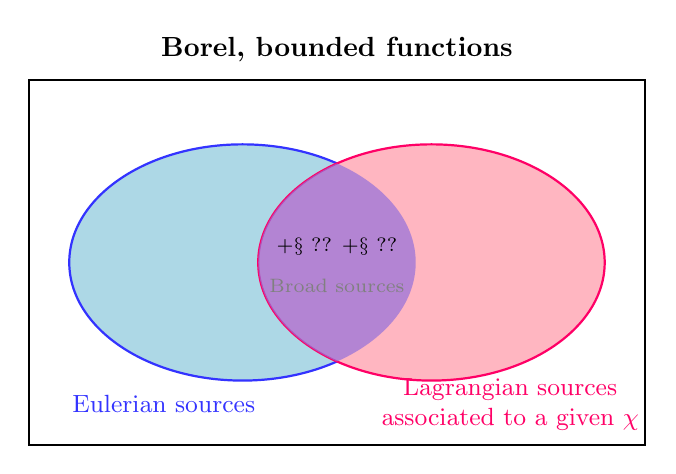
\begin{tikzpicture}[scale=1, every node/.style={font=\small}]

    % 定义颜色
    \definecolor{leftcolor}{RGB}{173, 216, 230}
    \definecolor{rightcolor}{RGB}{255, 182, 193}
    \definecolor{intersectcolor}{RGB}{147, 112, 219}
    
    % 绘制左椭圆 (Eulerian sources)
    \node[ellipse, minimum width=4.4cm, minimum height=3cm, 
          fill=leftcolor, draw=blue!80, thick] (left) at (-1.2, 0) {};
    
    % 绘制右椭圆 (Lagrangian sources)
    \node[ellipse, minimum width=4.4cm, minimum height=3cm, 
          fill=rightcolor, draw=red!60!magenta, thick] (right) at (1.2, 0) {};
    
    % 交集区域 (需要手动绘制或使用clip)
    \begin{scope}
        \clip (-1.2, 0) ellipse (2.2cm and 1.5cm);
        \fill[intersectcolor, opacity=0.7] (1.2, 0) ellipse (2.2cm and 1.5cm);
    \end{scope}
    
    % 数学表达式在交集中心
    \node[font=\scriptsize] at (0, 0.2) {$+\S$ ?? $+\S$ ??};
    \node[font=\scriptsize, color=gray] at (0, -0.3) {Broad sources};
    
    % 标签
    \node[font=\small, color=blue!80] at (-2.2, -1.8) {Eulerian sources};
    \node[font=\small, color=red!60!magenta, align=center] at (2.2, -1.8) 
          {Lagrangian sources\\associated to a given $\chi$};
    
    % 外框和标题
    \node[fit={(left) (right)}, draw=black, thick, 
          inner xsep=0.5cm, inner ysep=0.8cm] (frame) {};
    \node[above=0.1cm of frame.north, font=\normalsize\bfseries] 
          {Borel, bounded functions};
    
\end{tikzpicture}
\end{document}